
\section{Structural Induction}

The principle of mathematical induction is no doubt known to the
reader, not only as a proof technique, but also as a means of
constructing objects of a combinatorial nature. The idea of the proof
technique goes as follows. We want to know that a statement $P(n)$ is
true for all $n \ge 0$. Suppose we have proved $P(1)$ and $P(i)
\Rightarrow P(i+1)$. Then $P(n)$ is true because it appears in the
chain of implications $P(1) \Rightarrow P(2) \Rightarrow \cdots
\Rightarrow P(n) \Rightarrow \cdots$. The idea of the construction
technique is exemplified by the factorial function; to define $n!$ for
all $n \ge 1$ it suffices to define $1! = 1$ and $n! = n\cdot (n-1)!$.
The underlying mechanism which makes induction work is that there is a
family of statements (resp.~objects) which are indexed by the positive
integers $\Z_{>0}$ and we have an ordering on $\Z_{>0}$ which allows
us to deduce the sought statement (resp.~to construct the sought
object) in terms of integers which are smaller with respect to the
ordering.

We will often find ourselves in a more general situation. The set
which will index our statements and objects will not be the set of
integers, but some well-founded set $\Sigma$ (definition below). Part
of what makes this sort of proof difficult to understand and to devise
is that, unlike for $\Z_{>0}$, the partial order on $\Sigma$ which
comes with the well-foundedness property is often not explicitly
stated nor even particularly obvious, and since we only have a partial
order, we may have many induction hypotheses to assume and many
induction steps to prove.

\begin{defn} Let $\Sigma$ be a set together with a partial order
    $\prec$. $\Sigma$ is called \emph{well-founded} if every nonempty
    subset $S \subset \Sigma$ has a minimal element with respect to
    $\prec$ i.e. \[\exists m\in S, \text{ } \forall x\in S, \text{ } x
    \nprec m.\]
\end{defn}

\noindent \textbf{Principle of Structural Induction.} Let $\Sigma$ be
a well-founded set. In order to show that a statement $P(x)$ holds for
all $x\in \Sigma$ it suffices to show that if $P(y)$ is true for all
$y \prec x$ then $P(x)$ is true.

\begin{ap} To be convinced that this is a legitimate principle of
    proof, it suffices to consider a minimal counterexample to the family of
    statements $P(x)$ as $x$ varies through $\Sigma$.
\end{ap}

\begin{ap} The statement $P(y)$ is true for all $y \prec x$
    corresponds to the induction hypothesis and the proof that this
    hypothesis implies $P(x)$ corresponds to the the induction step in
    classical mathematical induction. But unlike the classical case
    there is no longer a single induction hypothesis step nor a single
    induction step. Likewise there may be many base cases; in terms of
    the partial ordering we can say that for each minimum with respect
    to $\prec$ there exists a base case to verify.
\end{ap}

\begin{rem} Structural induction is also known as Noetherian
    induction.
\end{rem}

\begin{eg} If $n\ge 8$ then $n$ can be written as $n = 3a+5b$ with
    $a,b \ge 0$.

\noindent \emph{Proof.} Write $P(n)$ for the statement that $n =
3a+5b$ with $a,b \ge 0$.

The base cases are $P(8), P(9), P(10)$ which are proved, respectively,
by $8=3+5, 9 = 3*3, 10 = 5*2$. Note very well that none of $P(i)$ is
true for $i=0,1,2,4,7$.

Suppose that $n\ge 10$ and that $P(11),\dots,P(n)$ are all true. We
shall prove $P(n+1)$. Since $n-2 \ge 8$ we have by assumption that
$P(n-2)$ is true, i.e.~$n-2=3a+5b$ for some $a,b \ge 0$. Thus $n+1 =
3(a+1)+5b$ with $a+1, b \ge 0$, as required. ///

This is not a classical mathematical induction because we required
multiple induction hypotheses; the preceeding proof is a structural
induction with respect to the well-founded set $\{n \in \Z_{>0} : n
\ge 8\}.$
\end{eg}

\begin{eg} We recursively define a tree.  A tree $T$ is \[T :=
    \begin{cases} \text{a single vertex called the \emph{root}, or}\\
        \text{a root } r, \text{ trees } T_1,\dots,T_m, \text{ and an edge
        from } r \text{ to the roots of each } T_i.
    \end{cases} \] We write $T=T(r)$ in the first case and
    $T=T(r,T_1,\dots,T_m)$ in the second case.\footnote{To be
    completely rigorous we should only define $A$-labelled trees where
    $A$ is a given set; an element $r$ which labels the root is then
    required to be an element of $A$. Without this requirement, one
    runs into the usual bevy of set theoretic paradoxes.}

    This definition provides us with a well-founded set over which we
    can perform structural induction. Namely, consider the set of all
    trees. We define a partial order by $T_\alpha \prec T_\beta$ if
    there exists a finite sequence $T_1, T_2, \dots T_m$ such that
    $T_1 = T(r_1,T_\alpha, \dots), T_2 = T(r_2, T_1,\dots), \dots, T_m
    = T(r_m, T_{m-1},\dots)$ and $T_m=T_\beta$.

    The well-foundedness is clear; given any set $S$ of trees, take
    for a minimal element the tree in $S$ with the smallest number of
    nodes (there are many choices for the minimal element; we only
    need one of them). In fact, what we have shown with this
    definition is that any chain with respect to $\prec$ has a unique
    minimal element.

    Now, to prove by structural induction a statement $P(T)$ is true
    for all trees $T$, we must first prove it for the base case $T(r)$
    and assume the induction hypotheses $P(T')$ for all trees $T'
    \prec T$, i.e.~for all trees $T'$ smaller than $T$. In fact, since
    $T=T(r,T_1,\dots,T_m)$ it suffices to assume
    $P(T_1),\dots,P(T_m)$.  Then we must show that $P(T)$ follows from
    these assumptions. Here is an example.

    \bigskip

    \noindent \emph{Every tree has one more node than it has edges.}

    \noindent \emph{Proof.} Write $n(T)$ for the number of nodes in
    $T$ and $e(T)$ for the number of edges. The statement $P(T)$ is
    $n(T) = e(T) + 1.$

    The base case is $P(T(r))$ in which we have $n(T(r)) = 1$ and
    $e(T(r)) = 0$.
    Now write $T=T(r,T_1,\dots,T_m)$. We have
    \begin{align*}
        n(T) & = 1 + \sum_{i=1}^m n(T_i) \\
        & = 1 + \sum_{i=1}^m (e(T_i)+1)\\
        & = 1 + m + \sum_{i=1}^m e(T_i) \\
        & = 1 + e(T)
    \end{align*} where the second equality is comes from the induction
    hypotheses and the last equality follows from the construction of
    $T(r,T_1,\dots,T_m)$. ///
\end{eg}

\begin{eg}\label{ArithExpr} We would like to define numerical
    expressions of the form $2,3, 2+3, 2\ast 3, 2\circledast 3,
    (2+3)\circledast 5, x+2, x\circledast n, \dots $ with the idea of
    writing a computer program which is capable of evaluating such
    expressions. Here, $n\circledast a = n^a$ signifies
    exponentiation.

    An \emph{expression} is defined recursively as follows. The basic
    expressions are numbers and letters. Intuitively, the letters
    stand for variables into which we may later substitute numbers.
    The recursive definition goes as follows:

    \begin{quote} If $E$ and $F$ are expressions then so are $E+F,
        E\ast F, E\circledast F, \text{ and } (E).$
    \end{quote}

    % holy shit, this contains all of algebraic geometry. . .

    Now that we have the definition of an expression, let us use
    structural induction to prove the following fact.

    \bigskip

    \noindent \emph{Every expression has an equal number of left and
    right parentheses.}

    \noindent \emph{Proof.} Given an expression $G$, write $l(G)$ for
    the number of left parentheses of $G$ and $r(G)$ for the number of
    right parentheses. Write $P(G)$ for the statement $l(G) = r(G)$.

    For a basic expression in which $G$ is just a number or a letter,
    $l(G)=r(G)=0$.

    Now we assume that $P(E), P(F)$ is true for all expressions $E,F$
    and must prove each of the following \[P(E+F), P(E\ast F), P(E
    \circledast F), P( ( E ) )  \] since these are all of the ways
    that $G$ could be built up from smaller expressions. In the first
    three cases we have $l(G) = l(E)+l(F) = r(E)+r(F) = r(G)$. In the
    last case we have $l(G) = l(E)+1$ and $r(G) = r(E)+1$. Thus in all
    cases we have proved that $l(G)=r(G)$. ///

    Observe that unlike the previous example we did not explicitly
    state the well-founded set nor the partial order on it. Often in
    such proofs, one omits mention of those two pieces of information.
    Nevertheless, it is best to know how to construct the underlying
    well-founded set with its partial order since that can be crucial
    to discovering a structural induction proof.
\end{eg}

\section{Finite State Automata}

In this section of the lecture notes, we closely follow chapter 1 of
``Word Processing in Groups'' by Epstein.

Some other references:

\begin{itemize}
    \item Hopcroft, Motwani, Ullman, Introduction to Automata Theory,
        Languages, and Computation (2e),
    \item Kozen, Automata and Computability,
    \item Sipser, Introduction to the Theory of Computation (2e).
\end{itemize}

\begin{defns} An \emph{alphabet} $A$ is simply a finite set.  A
    \emph{letter} is an element of $A$. A \emph{string} over the
    alphabet is a finite sequence of letters, or equivalently, a map
    $\{1, \dots, n\} \rightarrow A.$ If $n=0$ the domain is the empty
    set $\varnothing$ and there is a unique such string, denoted
    $\varepsilon$ and called the empty string. Typically, $A$ will be
    clear from the context, but we will occasionally write
    $\varepsilon_A$ instead of $\varepsilon$ in case of ambiguity.

    A nonempty string will be written by simply writing the succesive
    values left to right. Thus \texttt{00101110} is the representation
    of a map $\{1,\dots,8\}\rightarrow \{0,1\}.$ If $\omega$ is a
    string $\{1,\dots,n\} \rightarrow A$ then we call $n$ the
    \emph{length} of $\omega$, and denote it by $|\omega|$.

    We write $A^*$ for the set of all strings over $A$.
\end{defns}

\begin{defns} A \emph{semigroup} is a set $S$ together with a map $\mu
    : S\times S \rightarrow S$, such that $$\mu(\mu(a,b),c) =
    \mu(a,\mu(b,c)) \text{ for all } a,b,c\in S.$$ Usually we will
    write $a\cdot b$ or simply $ab$ for $\mu(a,b)$. A \emph{monoid}
    $M$ is a semigroup with a distinguished element $1\in M$ such that
    \[1\cdot a = a \cdot 1 = a \text{ for all } a\in M.\] A
    \emph{group} $G$ is a monoid together with an additional map $i :
    G \rightarrow G$, also written $i(a) = a^{-1}$, such that \[a
    a^{-1} = a^{-1} a = 1 \text{ for all } a \in G.\]
\end{defns}

\begin{egs} (a) The set $2\Z = \{\dots, -4, -2, 0, 2,4,\dots\}$ is a
    semigroup under multiplication and is a group under addition. It
    is not a monoid (and therefore not a group) under multiplication.

    (b) The set $\N = \{1,2,3,\dots\}$ is a monoid but not a group under
    multiplication and a semigroup but not a monoid under addition.

    (c) The set $\Q$ of rational numbers is a group under addition but
    only a monoid under multiplication. The set $\Q - \{0\}$ is a
    group under multiplication.

\end{egs}

\begin{defns} Given two strings $\omega: \{1,\dots,n\} \rightarrow A$
    and $\tau : \{1,\dots,m\} \rightarrow A,$ the \emph{concatenation}
    $\omega \tau$ of $\omega$ and $\tau$ is defined to be the string
    \(\{1,\dots,m+n\} \rightarrow A\) given by
    \[ (\omega\tau)(i) :=
        \begin{cases}
            \omega(i) & \text{if } 1 \le  i \le n, \\
            \tau(i-n) & \text{if } n + 1 \le i \le n+m.
        \end{cases} \] In other words, $\omega\tau$ is simply the
        result of writing out $\omega$ and then writing out $\tau$,
        left to right.

    If we have $w=puq$ for some (possibly empty) strings $w,p,q,u$
    over $A$. We say that $p$ is a \emph{prefix} of $w$, that $q$ is a
    \emph{suffix} of $w$, and that $u$ is a \emph{substring} of $w$.

    Given an integer $t\ge 0$ write $w(t)$ for that prefix of $w$ of
    length $t$, or $w$ itself if $t > |w|$.
\end{defns}

\begin{eg} Under concatenation of strings, $A^*$ is a monoid. We will
    see later that $A^*$ is in fact the free monoid on the set $A$.
\end{eg}

\begin{defn} A \emph{language} over $A$ is a subset of $A^*$. $A$ will
    usually be clear from the context and will not be mentioned.
    However, to be precise, we must take note of $A$. For instance, we
    must distinguish the the empty language over $\{x\}$ from the
    empty language over $\{x,y\}.$
\end{defn}

\begin{ap} For a language to be useful, there should be some way of
    understanding it. One way to interpret this requirement is to
    demand that there is some sort of machine capable of examining
    strings in $A^*$ and responding with a ``Yes'' if and only if the
    string is in the language under consideration. In this case we say
    that the machine recognizes or accepts the language. In general in
    theoretical computer science, the machine may or may not ever give
    an answer if the string is not in the language. More on this point
    later.
\end{ap}

\begin{defns} Let $U$ and $V$ be languages over $A$. Their
    \emph{concatenation} $UV$ is \[UV := \{uv \in A^* : u \in U, v \in
    V\}.\] The \emph{star closure} (also known as the \emph{Kleene
    closure}) of $U$ is \[ U^* := \bigcup_{n=0}^\infty U^n,\] where
    $U^0 := \{\varepsilon\}$ and $U^n = U^{n-1}U$ for $n>0$. If $U=A$
    then this agrees with our earlier definition of $A^*$.
\end{defns}

\begin{defn}\label{regexdef} Given a language $A$ we form the alphabet
    \Areg{} as follows.  Consider the set of five elements given by
    $$\Psi = \{(,), *, \vee, \varepsilon_\varnothing\}.$$   We
    pronounce $\vee$ as ``or,'' $*$ as ``star,'' and $\varnothing$ as
    ``null'' in this context. Let \[\Areg := A \sqcup \Psi \] be the
    disjoint union of $A$ and $\Psi.$ Note well the distinct meanings
    of the symbols $\varepsilon_\varnothing\in \Psi$,
    $\varepsilon_A\in A^*$, and $\varepsilon_{\Areg} \in \Areg^*.$

    The motivation for introducing these symbols goes as follows. The
    parentheses are to denote grouping, $*$ is to indicate repetition,
    $\vee$ is how we combine alternative patterns, and
    $\varepsilon_\varnothing$ matches the empty string $\varepsilon_A$
    of $A$.

    We now inductively define a \emph{regular expression} over $A$,
    which is a certain type of string over \Areg, and \emph{regular
    languages} which are certain languages over $A$ associated to
    regular expressions, as follows.

    (1) $\varepsilon_\varnothing$ is a regular expression
    which gives rise to the language $L(\varepsilon_\varnothing) =
    \{\varepsilon_A\}$,

    (2) $a$ is a regular expression for $a\in A$ and $L(a) = \{a\}$,

    (3) $()$ is a regular expression and $L( ( ) ) = \varnothing$.

    (4) If $r$ is a regular expression then $(r)$ is a regular
    expression, and $L( ( r) ) := L(r)$.

    (5) If $r$ is a regular expression then $(r^*)$ is a regular
    expression which gives rise to the language $L( (r^*) ) =
    (L(r))^*.$

    (6) If $r$ and $s$ are regular expressions then so is $(r\vee s)$
    and the latter gives the language $L( (r \vee s) ) = L(r)\cup L(s)$.

    (7) If $r$ and $s$ are regular expressions then so is $(r s)$
    and the latter gives the language $L( (r s) ) = L(r)L(s)$.

    All regular expressions arise by being built up from the primitive
    expressions (1),(2),(3) by means of the rules (4),(5),(6),(7). If $r$
    is a regular expression and $w\in L(r)$ then we say that $w$
    \emph{matches} $r$.

    Note well: this recursive definition enables us to use structural
    induction over the set of regular expressions. See example
    \ref{ArithExpr}.
\end{defn}

\begin{rems}
    (1) The languages $L(a)$ and $L(\varepsilon_\varnothing)$ have
    one element each and the language $L( ( ) )$ has no elements.

    (2) The assignment $r\mapsto L(r)$ from regular expressions to
    regular languages is far from injective.

    (3) If $r = a \in A$ then $L( (a^*) ) = \{\varepsilon_A, a, a^2,
    a^3, \dots\}.$

    (4) Often, we will omit the parentheses when writing out regular
    expressions, in analogy with familiar rules from arithmetic: $*$
    is a sort of exponentiation which has a higher precedence than
    $\vee,$ the latter being the analogue of multiplication.
\end{rems}

\begin{prop} The set of languages over $A$ forms a monoid under
    concatenation. The identity element is the language whose only
    element is the empty string. The set of regular languages over $A$
    forms a submonoid. The set of finite languages (i.e.~the languages
    consisting of finite subsets of $A$) form a submonoid of the
    monoid of regular languages.
\end{prop}
\begin{proof} Unwind the definitions.
\end{proof}

\begin{defn} A \emph{finite state automaton} (or simply
    \emph{automaton}) over $A$ is a quintuple $$(S,A,\mu,Y,s_0)$$
    consisting of

    (1) a finite set $S$, called the set of \emph{states},

    (2) a finite set $A$, called the \emph{alphabet},

    (3) $\mu : S\times A \rightarrow S$ is a mapping, called the
    \emph{transition function},

    (4) $Y \subset S$ is a possibly empty set of \emph{accept states}, and

    (5) $s_0$ is the \emph{start} or \emph{initial} state.

    We usually suppress $\mu$ from the notation and write $sx =
    \mu(s,x).$
\end{defn}

\begin{rem} The letter $Y$ stands for ``Yes.'' The motivation for this
    definition is as follows. We are given a string $\omega = a_1\dots
    a_n$ over $A$ which we imagine to be printed left to right on a
    tape. The first letter tells us where to go from $s_0$: $s_1 = s_0
    a_1$ The next letter tells us where to go from $s_1$: $s_2 = s_1
    a_2$. And so on. If, after consuming all of $w$, the final state
    $s_n$ is in $Y$, we interpret the machine as having said ``Yes''
    in answer to a question about the given string $w$. We now proceed
    to make these ideas precise.
\end{rem}

\begin{defns} Let $M = (S,A,\mu,Y,s_0)$ be a finite state automaton
    and let \End{S} be the monoid of all set theoretic maps
    $S\rightarrow S$. The map $A\rightarrow \End{S}$ may be extended
    in a unique way to a monoid homomorphism \[A^* \rightarrow
    \End{S}.\] We say that a string $w$ is \emph{recognized} or
    \emph{accepted} by $M$ if the corresponding element of $\End{S}$ takes
    $s_0$ to $Y$. The set \[L(M) := \{w \in A^* : w \text{ is recognized
    by } M\}\] is called the language recognized by $M$, or simply the
    \emph{language of $M$. }
\end{defns}

\begin{rem} We may express the definition as follows. Let $a\in A$.
    Then we define a function $f_a : S\rightarrow S$ by $f_a(x) :=
    \mu(x,a).$

    Some notation: for any mappings $f: X \rightarrow Y$ and $g : Y
    \rightarrow Z$ we write $f;g = g \circ f$ so that for all $x\in X$
    we have $(f;g)(x) = g(f(x))$.

    Now, let $w = a_1\cdots a_n \in A^*$. Then we define a map $f_w :
    S \rightarrow S$ by $$f_w = f_{a_1} ; f_{a_2} ; \cdots ;
    f_{a_n}.$$

    If we write $\mu(x,a) = xa$ then the above is simply expressing \[
    x(a_1\cdots a_n) = ( ( ( (x a_1)a_2)\cdots a_n)\cdots) \] and the
    associativity of $A^*$ and of \End{S} guarantees that it makes no
    difference how we arrange the parentheses. (By using the language
    of monoids and their homomorphisms, we don't have to explicitly
    mention associativity.)

    Very shortly we will study homomorphisms and the extension of maps
    from $A$ to the free monoid generated by $A$.
\end{rem}

\begin{ap} We draw a finite state automaton by means of a finite
    directed graph. The set of vertices is the set $S$ of states, and
    the set of directed edges is the set of pairs $\{(s,\mu(s,a)) : a
    \in A\}.$ The subset of accept states, $Y \subset S$, is indicated
    by a double circle around that vertex and the initial state is
    indicated by a wavy arrow. See the figure.

    \begin{center}
    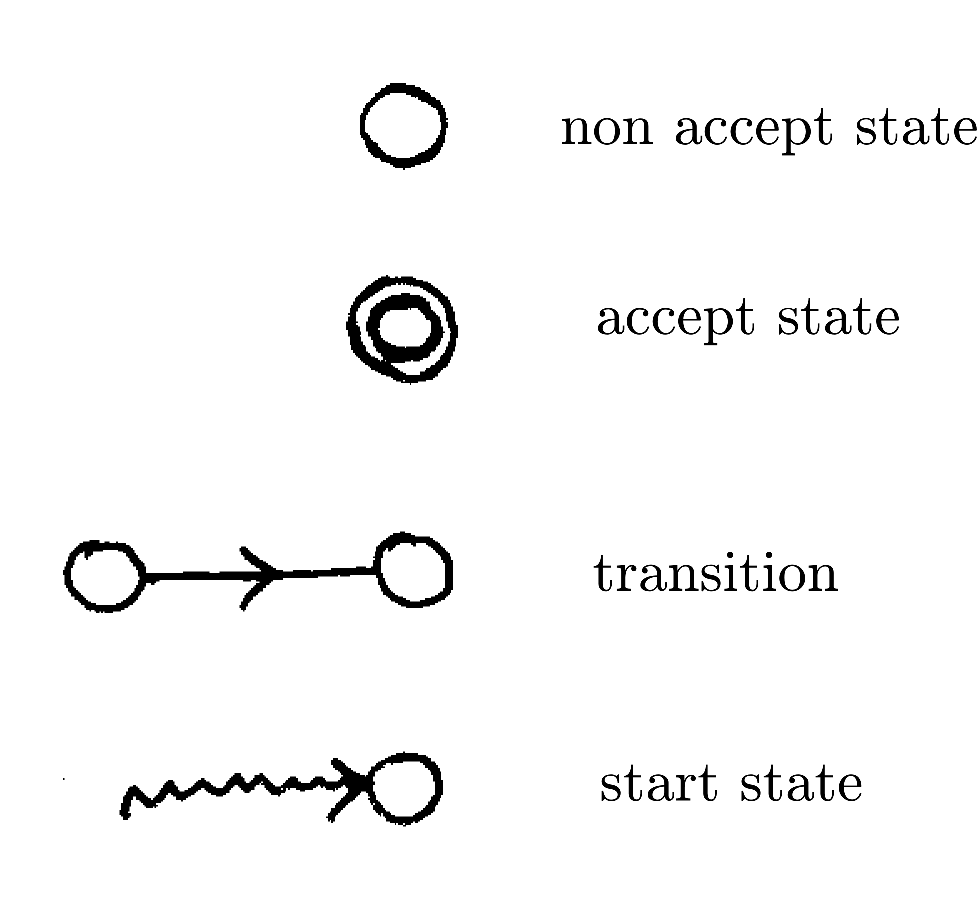
\includegraphics[scale=0.35]{resources/vertices-on-automata.pdf}
    \end{center}
\end{ap}

\begin{eg} The alphabet in this case is $\mathtt{\{1,+\}}.$
    %The displayed automaton computes the function $f(x) = x + 1
    %\imod{3}$ (exercise for the reader: make sense of the domain
    %and range of $f$).
    \begin{center}
        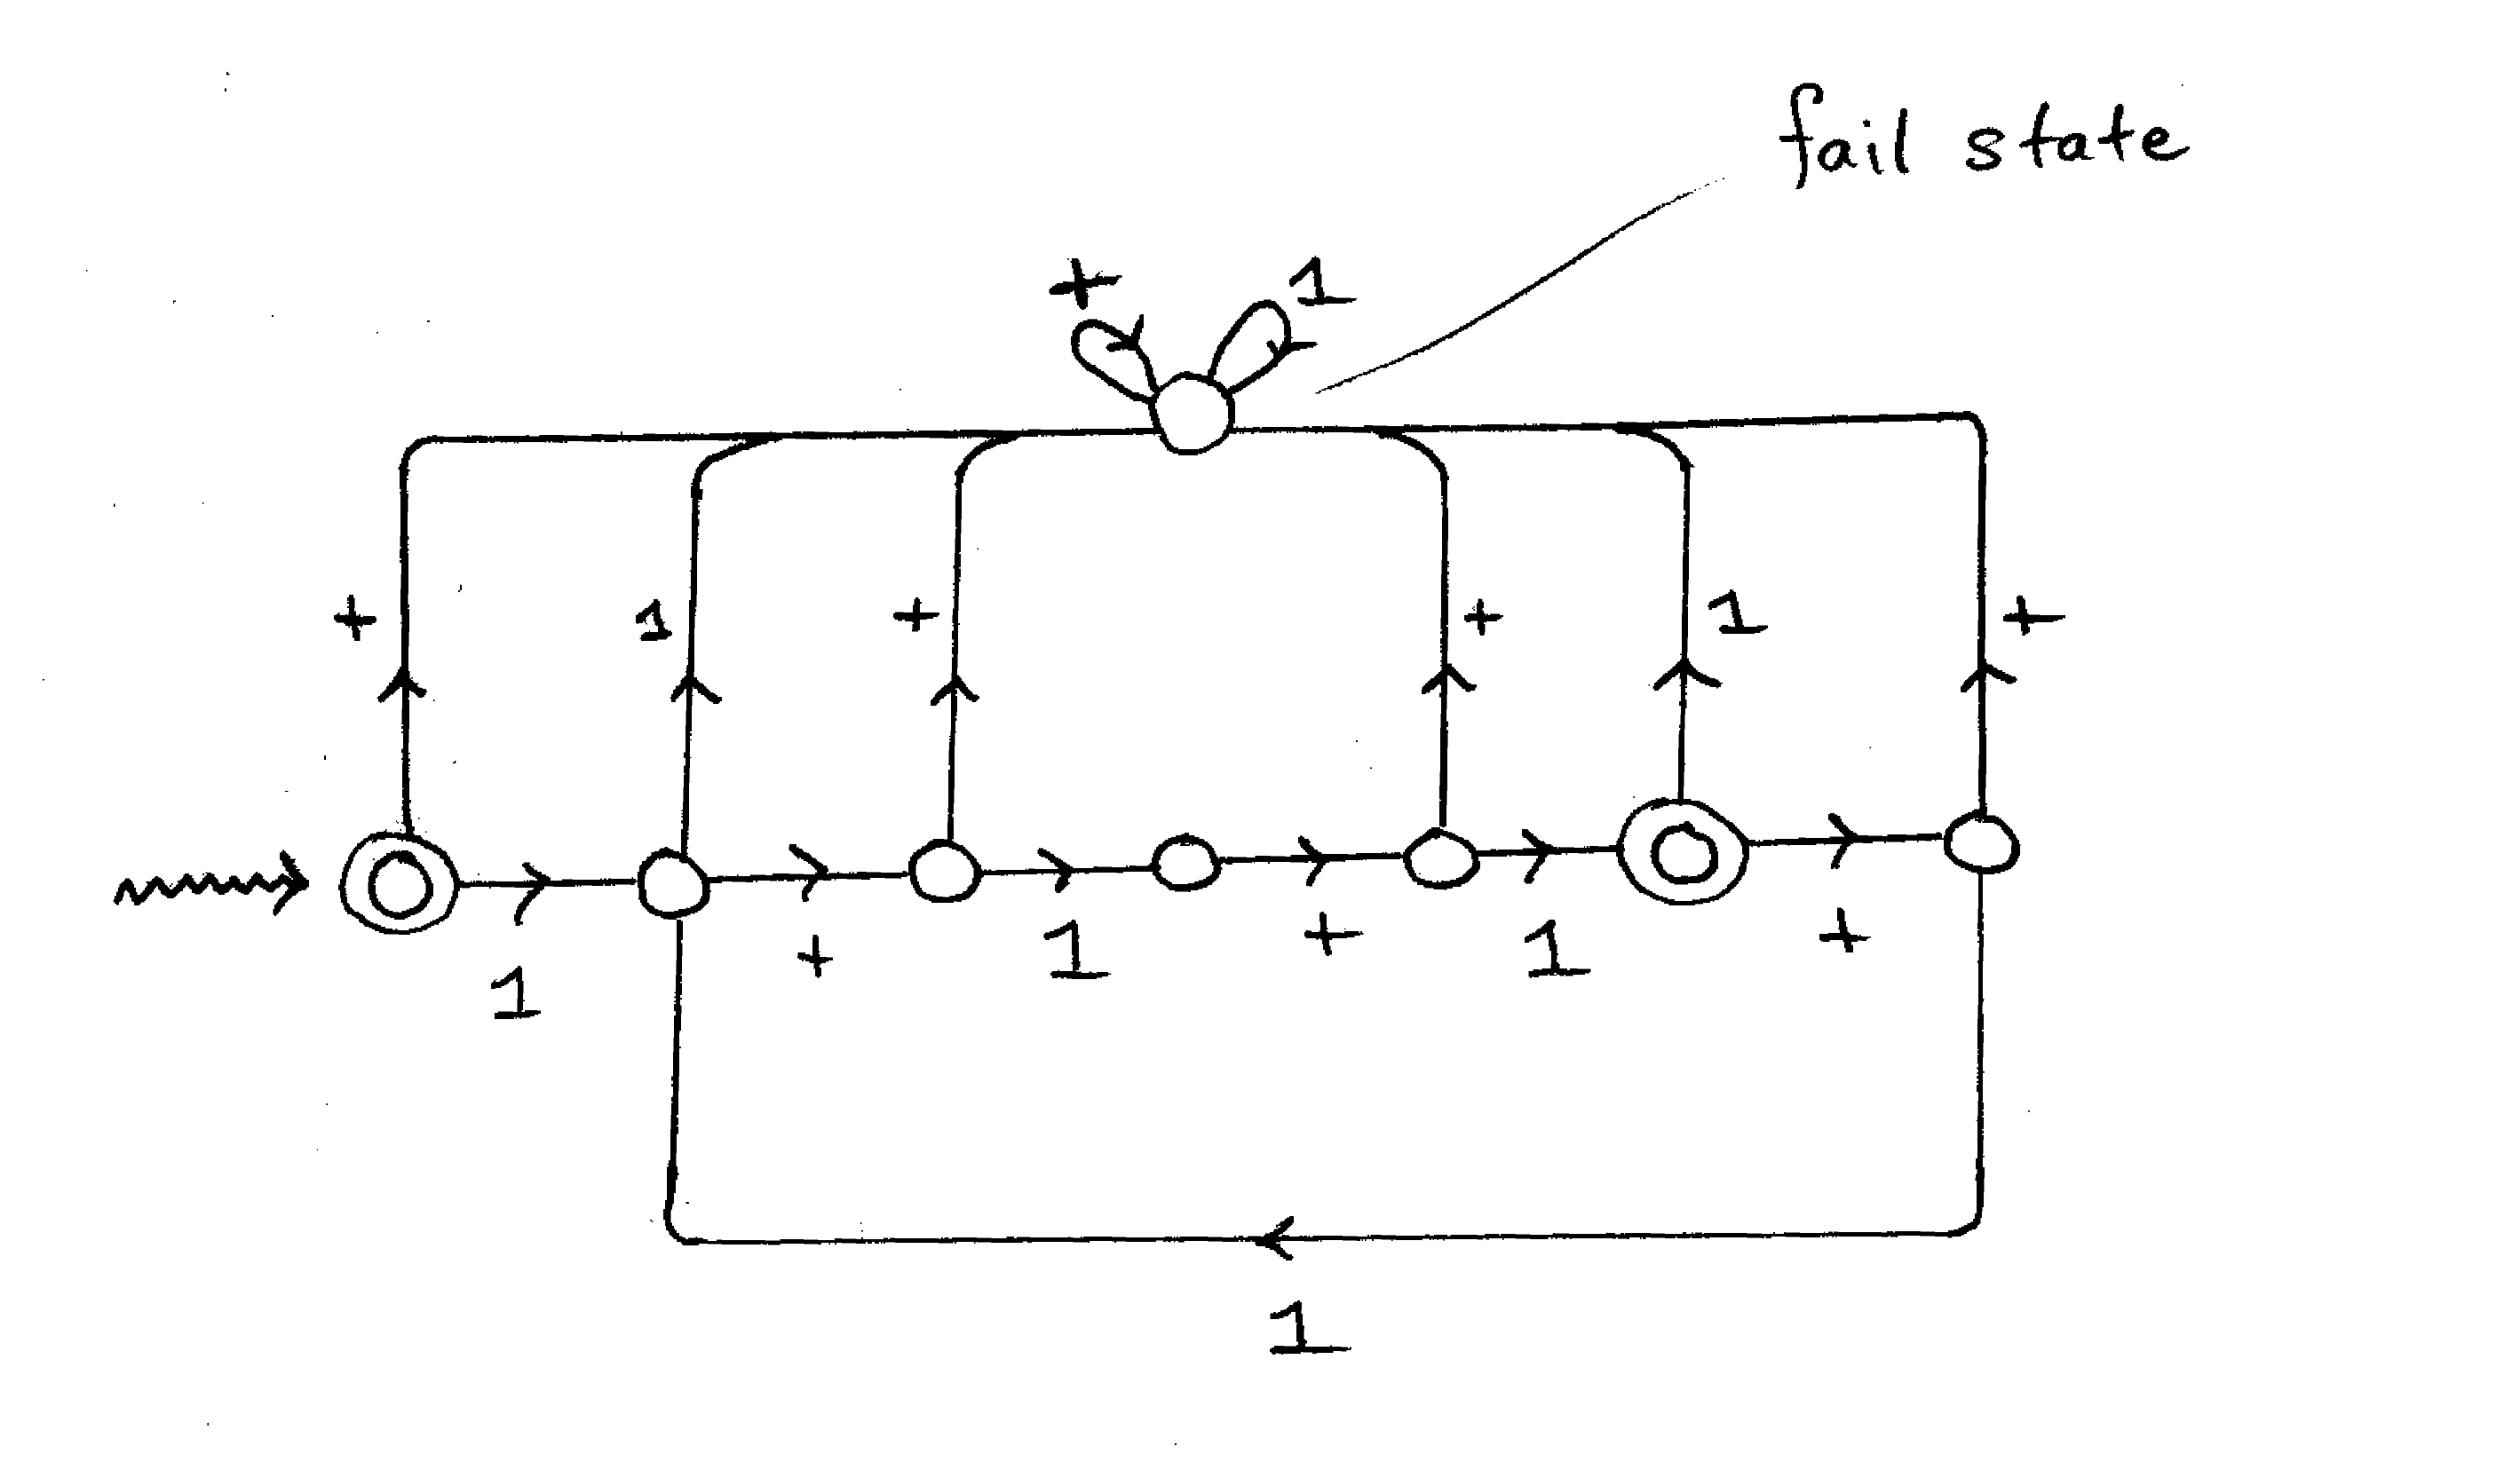
\includegraphics[scale=0.25]{resources/plus-1-mod-3.pdf}
    \end{center}
\end{eg}

\begin{ap} We can often transform a finite state automaton to a
    simpler one without changing the language it recognizes, as
    follows. (1) Remove all of the automaton's \emph{inaccessible
    states}, those that cannot be reached from the start state by
    traversing a sequence of edges. (2) A state is called \emph{live}
    or \emph{dead} according as there is or isn't an accept state that
    can be reached from it. (Observe: it is possible for a state to be
    both live and inaccessible.) We collapse all of the automaton's
    dead states into a single \emph{failure state} which is by
    definition a vertex which transitions to no states other than
    itself and is not an accept state.

    An automaton is said to be \emph{normalized} if the above
    procedure has already been applied to it. Henceforth we will only
    work with normalized automata.
\end{ap}

\begin{ap} A finite state automaton is also known as a
    \emph{deterministic finite state automaton}. An \emph{arrow} is a
    triple $(s,\alpha,t)$ where $s,t \in S$ and $\alpha$ is called the
    \emph{label} of the arrow. $\alpha$ may come from any set, $s$ is
    called the source of the arrow, and $t$ the target of the arrow.
    An arrow labelled by $\alpha$ is also called an
    \emph{$\alpha$-transition.}
\end{ap}

\begin{defn} A \emph{nondeterministic finite state automaton} is a
    quintuple $$(S,A,\mu,Y,S_0)$$ where

    (1) the \emph{alphabet} $A$ is a
    finite set,

    (2) the \emph{state set} $S$ is another finite set,

    (3) $S_0 \subset S$ is the set of \emph{start states},

    (4) $Y \subset S$ is the set of \emph{accept states}

    (5) $\mu$ is a set of arrows with labels in the set $A\sqcup
    \{\varepsilon\}$ (disjoint union; $\varepsilon$ is to be thought
    of as an empty string).
\end{defn}

\begin{ap} Thus the differences between a nondeterministic automaton
    and an automaton (= deterministic automaton) are as follows.

    (1) There are multiple points of entry: the single start state
    $s_0$ has been replaced by a set of start states $S_0$.

    (2) It is possible to leap between states without consuming an
    element of $A$; this is what it means to have an arrow labelled by
    $\varepsilon.$

    (3) The function $\mu : S\times A \rightarrow S$ has been replaced
    by a relation on the set of states. Recall that a relation is a
    subset of the set of pairs: $R \subset S\times S$. A function is a special
    type of relation which satisfies ``the vertical line test''
    familiar from calculus. Thus, saying that $\mu$ is a set of arrows
    with labels in $A\sqcup \{\varepsilon\}$ means that we have a
    relation $R \subset S\times S$ and a map $R \rightarrow A\sqcup
    \{\varepsilon\}$ which gives the labels.

    For concreteness, suppose that we have states $S = \{s,t,u\}$ and
    alphabet $A=\mathtt{\{a,b,c\}}$. The figure on the left is what a
    deterministic automata looks like, and the figure on the
    right is what a nondeterministic automata could look like.

    \begin{center}
        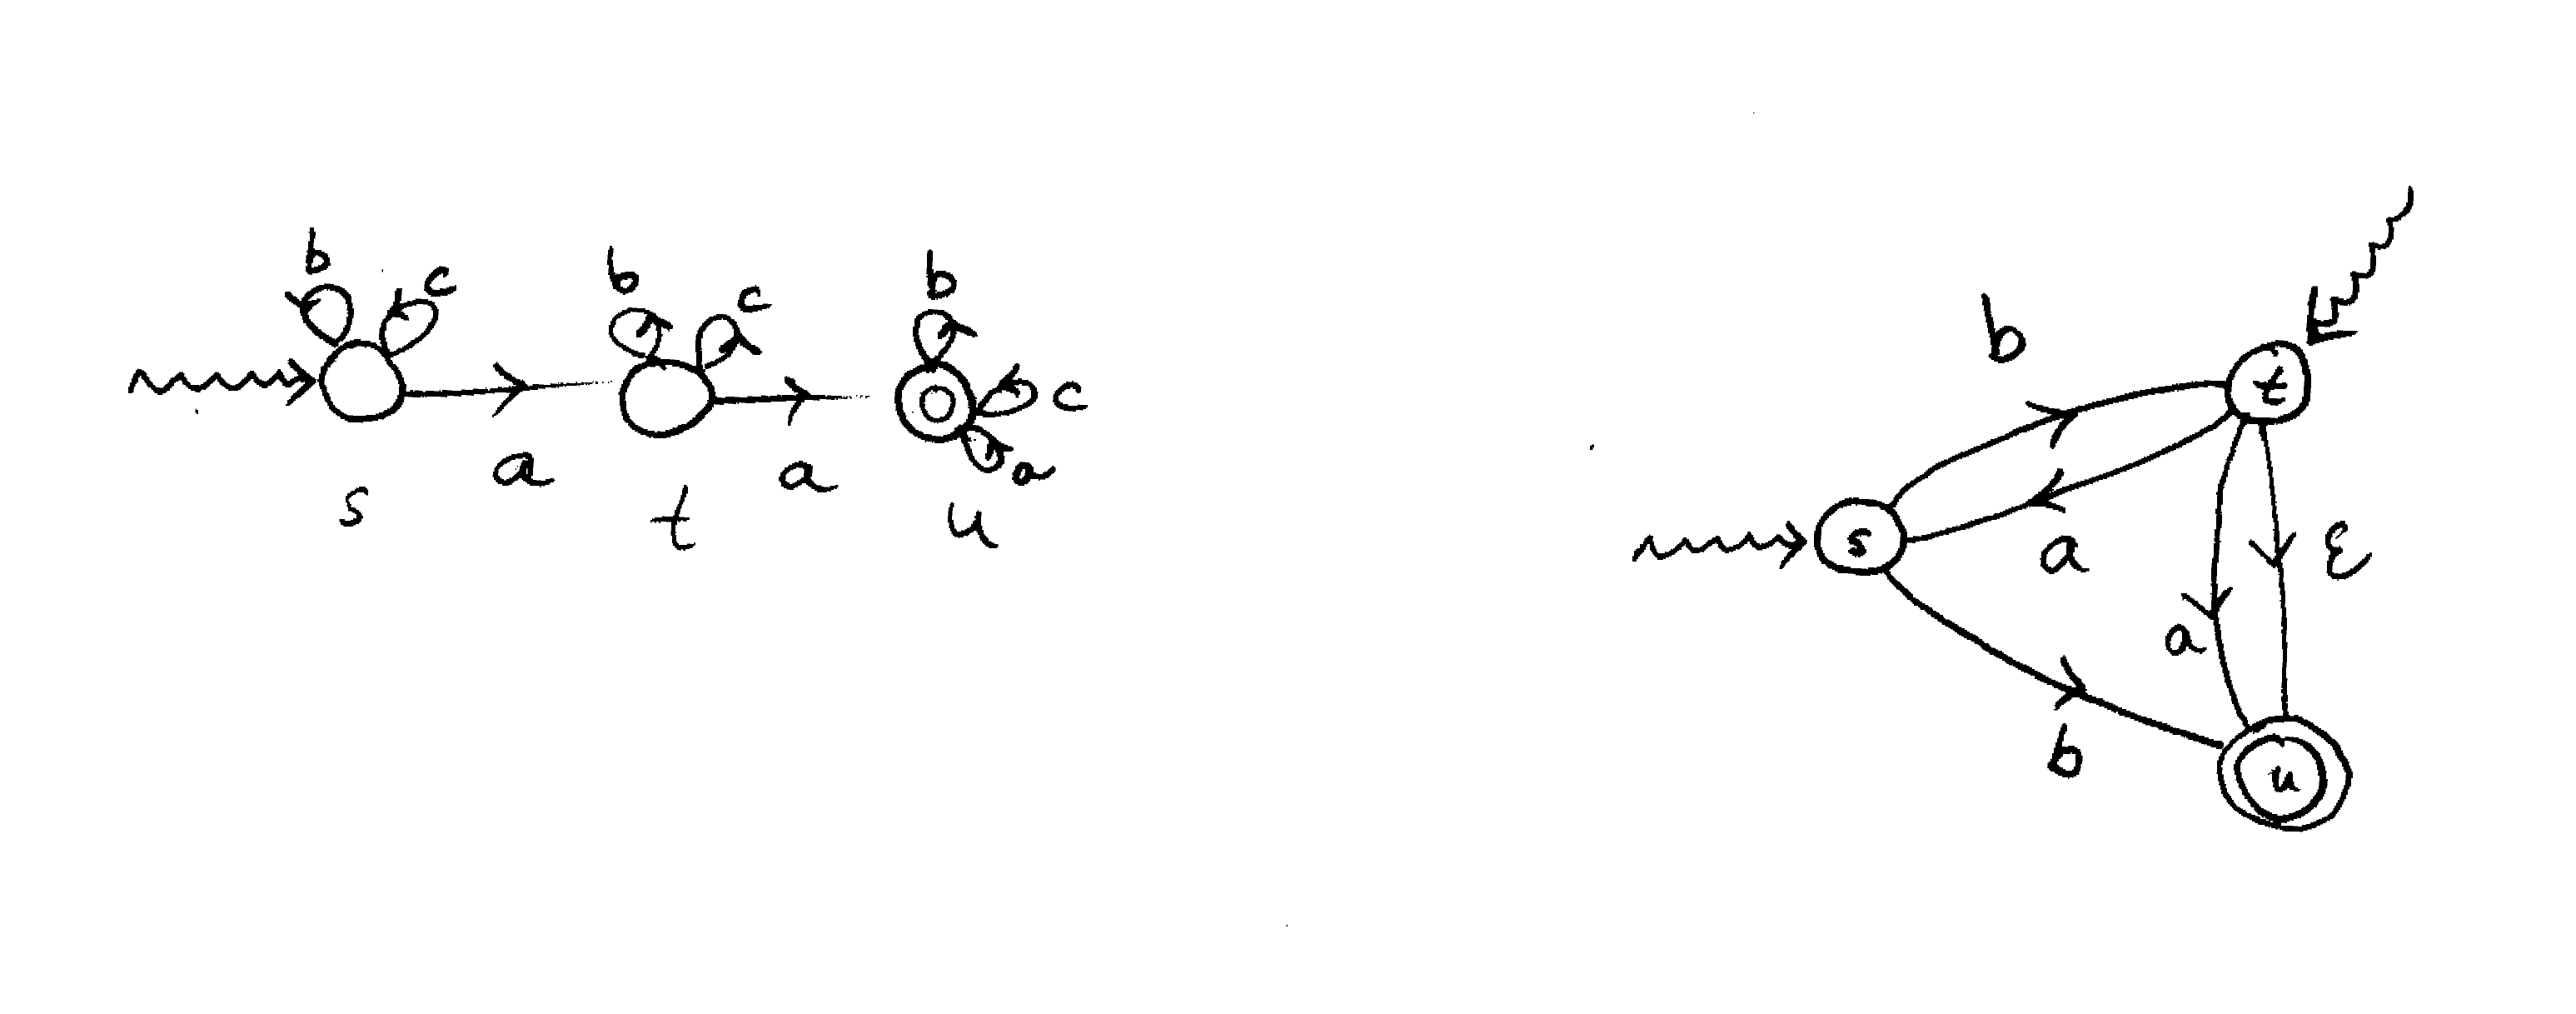
\includegraphics[scale=0.2]{resources/DFA-vs-NFA.pdf}
    \end{center}

    Moreover, we are to interpret the labels as telling us which of
    several possibilities we may take. For instance, if we are at
    state $t$, the label \texttt{a} on the figure on the right only
    tells us that there are two choices for the next step; thus the
    next step is not determined. In the figure on the left, the label
    \texttt{a} does determine our next step, from any given state.
\end{ap}

    \begin{center}
        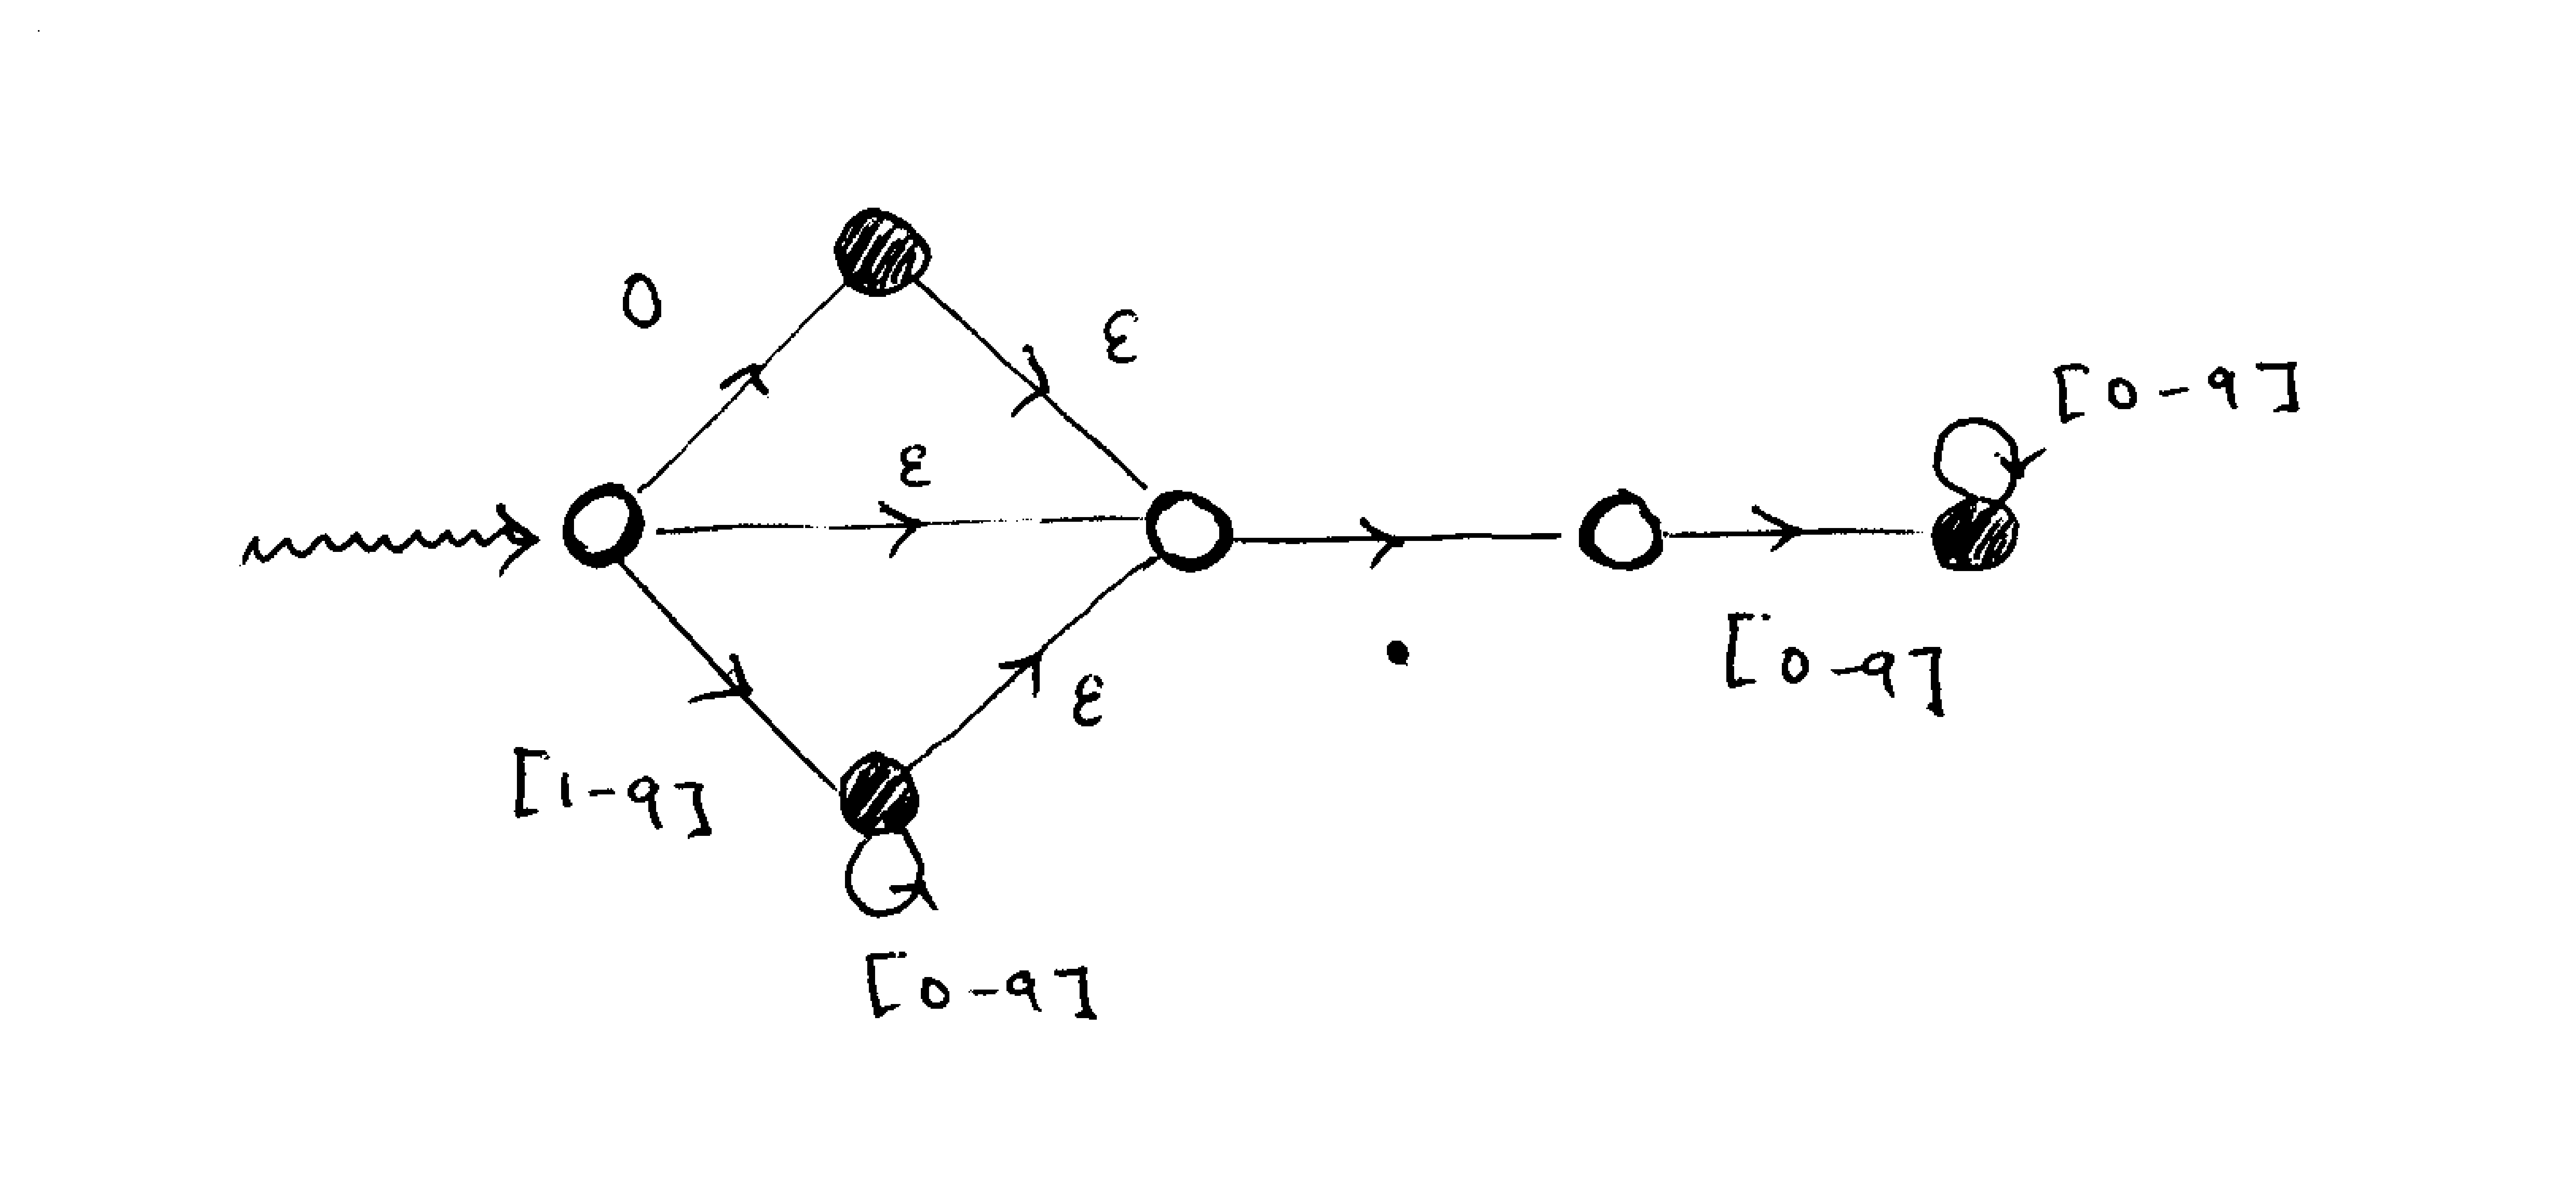
\includegraphics[scale=0.1]{resources/decimal-NFA.pdf}
    \end{center}

\begin{eg}
    The alphabet for the nondeterministic automaton of this figure is
    $$\mathtt{\{0,1,2,3,4,5,6,7,8,9,.\}}$$ consisting of eleven
    symbols. The only nondeterminism in this example is the use of
    $\varepsilon$-transitions. The other source of nondeterminism,
    which is not present in this example, is the possible entry to the
    automaton from one of several start states --- as with the
    $\varepsilon$-transition, that start state is not determined by
    the automaton, hence the adjective nondeterministic.
\end{eg}

\begin{defns} A \emph{generalized finite state automaton} is defined
    in the same way as a nondeterministic finite state automaton
    except that each edge is now labelled by a regular expression over
    $A$ instead of simply by an element of $A$.  Let $M$ be a
    generalized finite state automaton. We seek to define the language
    $L(M)$ \emph{recognized}, or \emph{accepted} $M$.

    A \emph{path of arrows} in $M$ is defined to be a sequence \[P =
    (s_1,u_1,s_2,u_2,\dots,u_n,s_{n+1})\] where $n\ge 0$ is the called
    the \emph{length} $\ell(P)$ of the path and each $u_i$ is the
    label of an arrow $(s_i,u_i,s_{i+1})$ with source $s_i$ and target
    $s_{i+1}$ as defined earlier. $s_1$ is called the \emph{source}
    and $s_{n+1}$ the \emph{target} of the given path of arrows. Given
    a path $P$ we will also write $s(P)$ and $t(P)$ for the source and
    target of $P$, respectively. Now, each $u_i$ is given by a regular
    expression. Let $w$ be the concatenation of these regular
    expressions, $w=u_1 \cdots u_n$.  Thus $w$ is a regular
    expression, which we call the \emph{label} of the given path, and
    it has an associated regular language $L(w)$. Finally we define
    $L(M) \subset A^*$ by \[L(M) := \bigcup_{P\in \mathscr{P}(S_0,Y)}
    L(w(P)) \] where $\mathscr{P}(S_0,Y)$ is the set of paths with
    source in $S_0$ and target in $Y$, $S_0$ and $Y$ came with the
    given automaton $M$, and $w(P)$ is the label associated to the
    path $P$.

    The foregoing equally well defines the language accepted by a
    nondeterministic finite automaton, where we regard each element of
    the $A$ as a regular expressions over $A$. Put differently, a
    nondeterministic finite automaton is also a generalized finite
    automaton in a natural way.
\end{defns}

\begin{defn} Given a nondeterministic automaton $M$ with state set $S$
    we define the \emph{$\varepsilon$-topology} on $S$ as follows.
    Let $x\in S$ and put \[Z_{x} := \left\{ t(P) : P \text{ is a path
    of arrows s.t. } s(P) = x \text{ and } w(P) =
    \varepsilon^{\ell(P)} \right\} \] and for $E \subset S$ put \[Z_E
    := \bigcup_{x\in E} Z_{x}.\] Considering paths of length zero, it
    is clear that $E \subset Z_E$. Since $S$ is a finite set, this
    definition realizes all closed sets in a topology on $S$.
\end{defn}

\begin{thm}[Kleene, Scott, Rabin] Let $A$ be an alphabet. The
    following conditions on a language over $A$ are equivalent.

    (a) The language is recognized by a finite state automaton.

    (b) The language is recognized by a nondeterministic finite state automaton.

    (c) The language is recognized by a generalized finite state automaton.

    (d) The language is defined by a regular expression.
\end{thm}

\begin{proof} We have (a) $\Rightarrow$ (b) $\Rightarrow$ (c) by
    definition.

    We now show that (c) $\Rightarrow$ (d). We are given a generalized
    finite state automaton with states $S$, start states $S_0$, and
    accept states $Y$. Given a path of arrows
    $(s_1,u_1,\dots,u_n,s_{n+1})$, say that it visits the states
    $s_2,\dots,s_n$ (observe that the path needn't visit its own
    source and target). Let $s_1,s_2 \in S$ and $X\subset S$ and
    define $L(s_1,s_2,X) := \bigcup L(w(P))$ where the $P$ range over
    those paths with source $s_1$, target $s_2$, and visiting only
    states in $X$. We shall show by induction on $\#X$ that
    $L(s_1,s_2,X)$ is defined by a regular expression.

    First suppose that $X=\varnothing$ so that $L(s_1,s_2,X)$ is
    simply the finite set of arrows with source $s_1$ and target
    $s_2$. Let $r_i (i = 1, \dots ,k)$  be the label of the $i$th
    arrow; $r_i$ is a regular expression. Then, recalling that $\vee$
    of regular expressions corresponds to $\bigcup$ of languages,  we
    have
    \[ L(s_1,s_2,X) =
    \begin{cases}
        L(r_1 \vee r_2 \vee \cdots \vee r_k) & \text{if } k > 0\\
        \varnothing & \text{if } k=0 \text{ and } s_1 \neq s_2\\
        \{\varepsilon\} & \text{if } k=0 \text{ and } s_1 = s_2
    \end{cases} \] so that $L(s_1,s_2,\varnothing)$ is indeed defined
    by a regular expression.

    Now suppose that $X\neq \varnothing$ and let $s\in X$. Put
    \begin{align*}
        L_1 & = L(s_1,s_2,X - \{s\}) \\
        L_2 & = L(s_1,s  ,X - \{s\}) \\
        L_3 & = L(s  ,s  ,X - \{s\}) \\
        L_4 & = L(s  ,s_2,X - \{s\}).
    \end{align*} Then we have that \[L(s_1,s_2,X) = L_1 \cup
    (L_2L_3^*L_4).\] The induction hypothesis guarantees us that each
    of the terms on the rhs is defined by a regular expression, and
    thus so too is $L(s_1,s_2,X)$. To complete the proof that (c)
    implies (d), observe that we have \[L(M) = \bigcup_{\substack{s_1
    \in S_0,\\ s_2\in Y}} L(s_1,s_2,S).\] Thus $L(M)$ is a finite
    union of languages each defined by a regular expression and we are
    done.

    We now seek to prove (d) $\Rightarrow$ (b). We shall use
    structural induction to construct a nondeterministic finite state
    automaton $M$ which accepts the same language as the given regular
    expression $R$. In all cases, let the automaton $M$ have as start
    states $S_0$ the singleton set $\{s_0\}$ and as accept states $Y$
    the singleton set $\{y\}$ with $s_0 \neq y$.

    If the regular expression if $()$ then the associated language is
    the empty language and the automaton has only the start state and
    accept state as vertices, with no arrows at all.

    If the regular expression is a single symbol $x\in A\cup
    \{\varepsilon\}$ then the automaton consists of a single arrow
    labeled by $x$ going from the start state to the accept state.
    The start and accept are the only states in this case as well.

    If $r$ is a regular expression corresponding to the machine $M$
    (this is a structural induction hypothesis) then we may construct
    a machine corresponding to $r^*$ as follows.  Create a single new
    $\varepsilon$-arrow from the accept state of $M$ to the start
    state.

    \begin{center}
        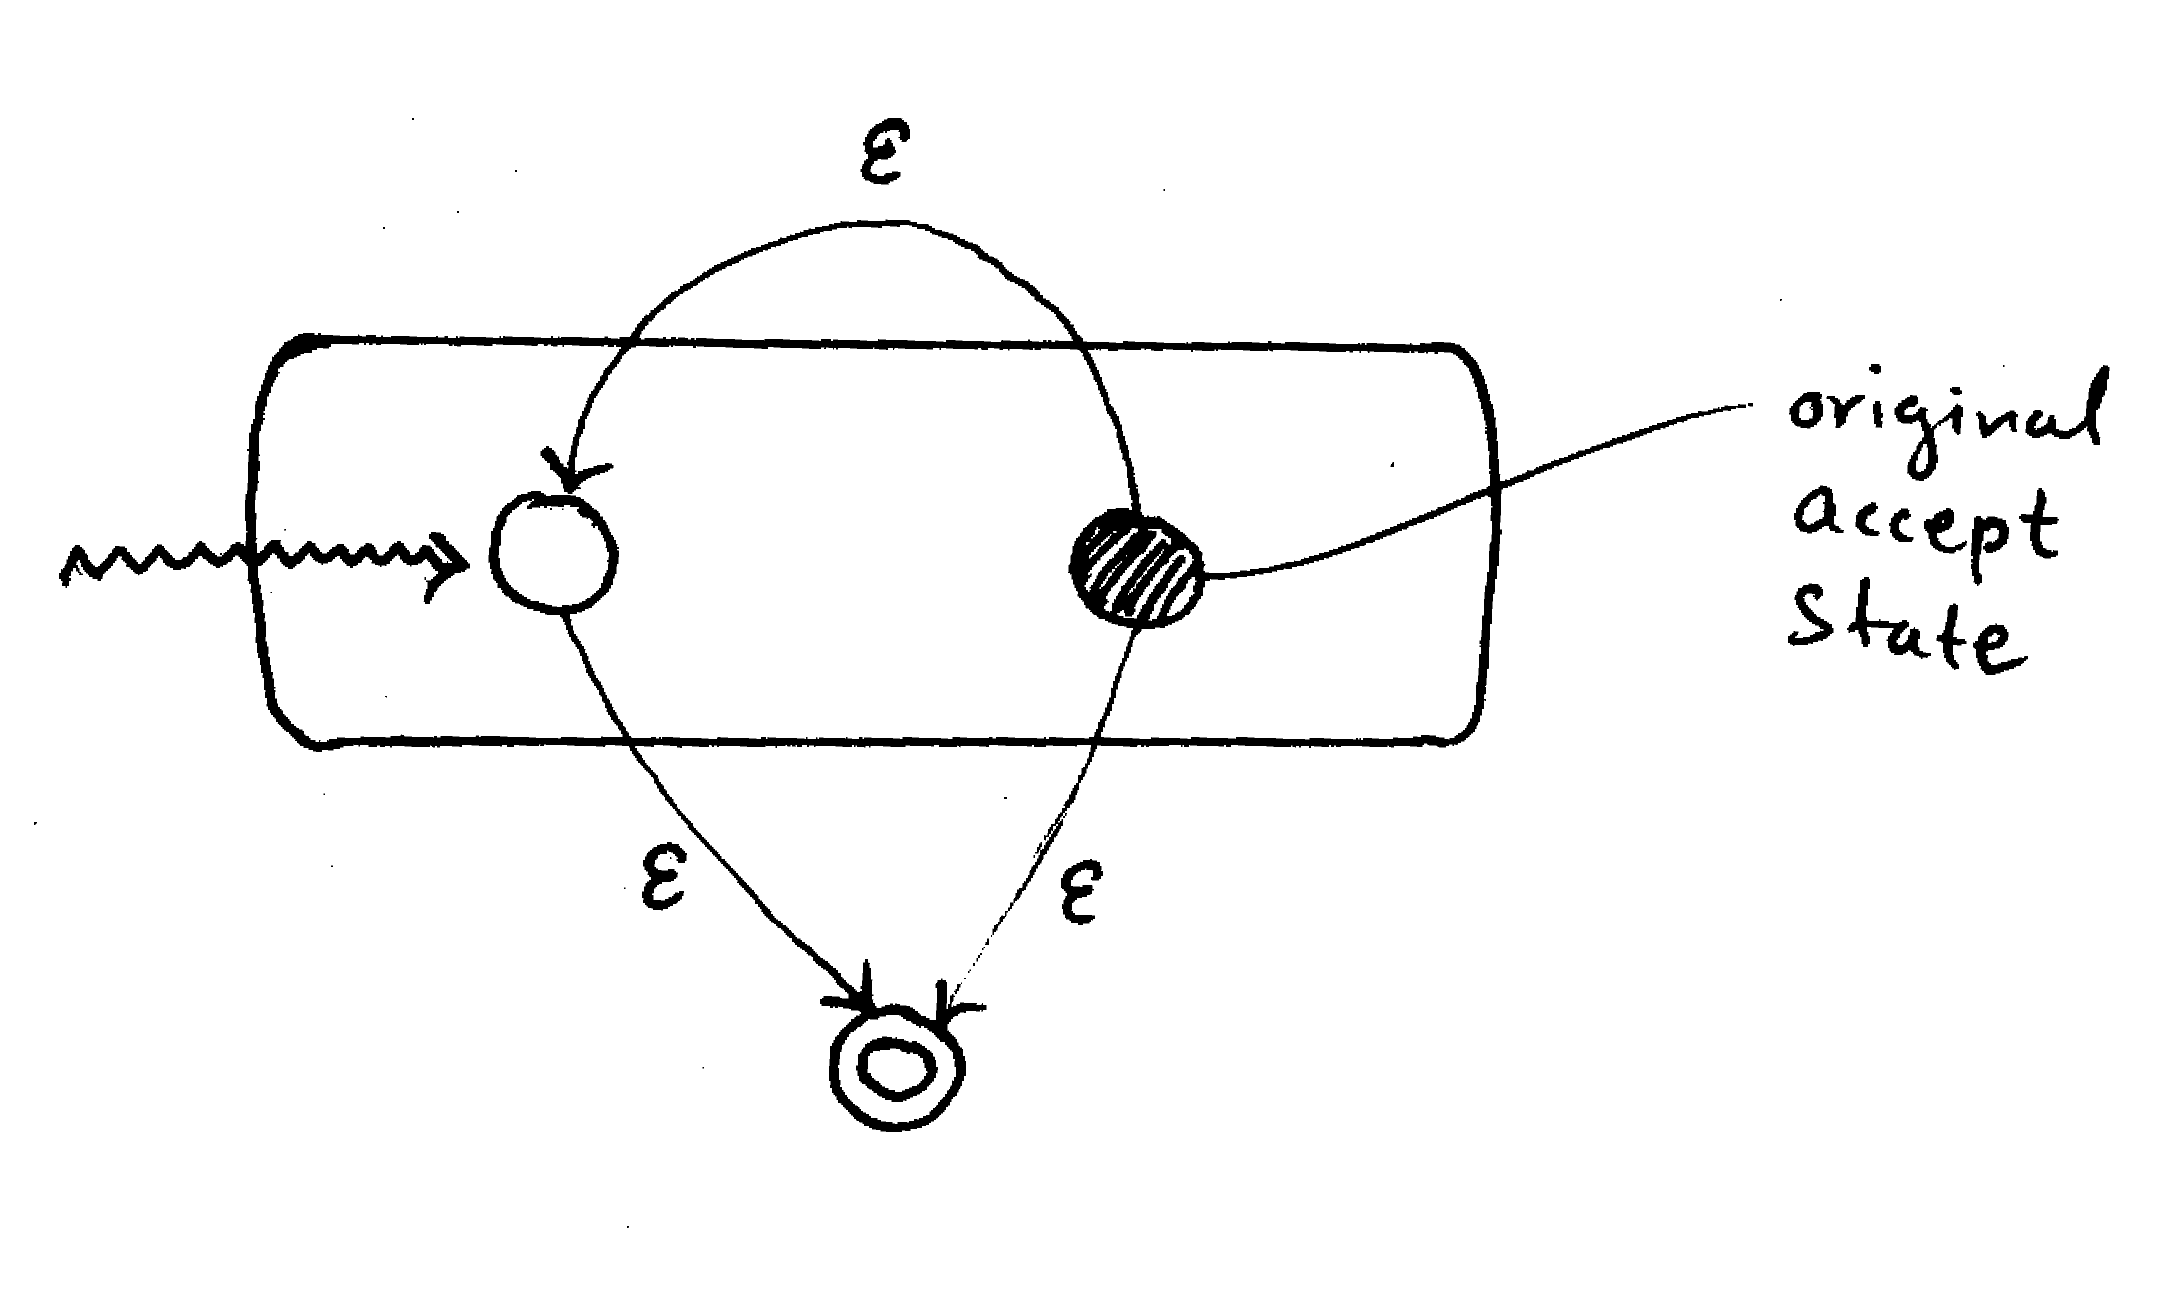
\includegraphics[scale=0.2]{resources/1-7.pdf}
    \end{center}

    If $r_1$ and $r_2$ are two regular expressions accepted by
    nondeterministic automata $M_1$ and $M_2$ (again this is a
    structural induction induction hypothesis) then the following
    figure gives the automata which accepts the concatenation $r_1
    r_2$.

    \begin{center}
        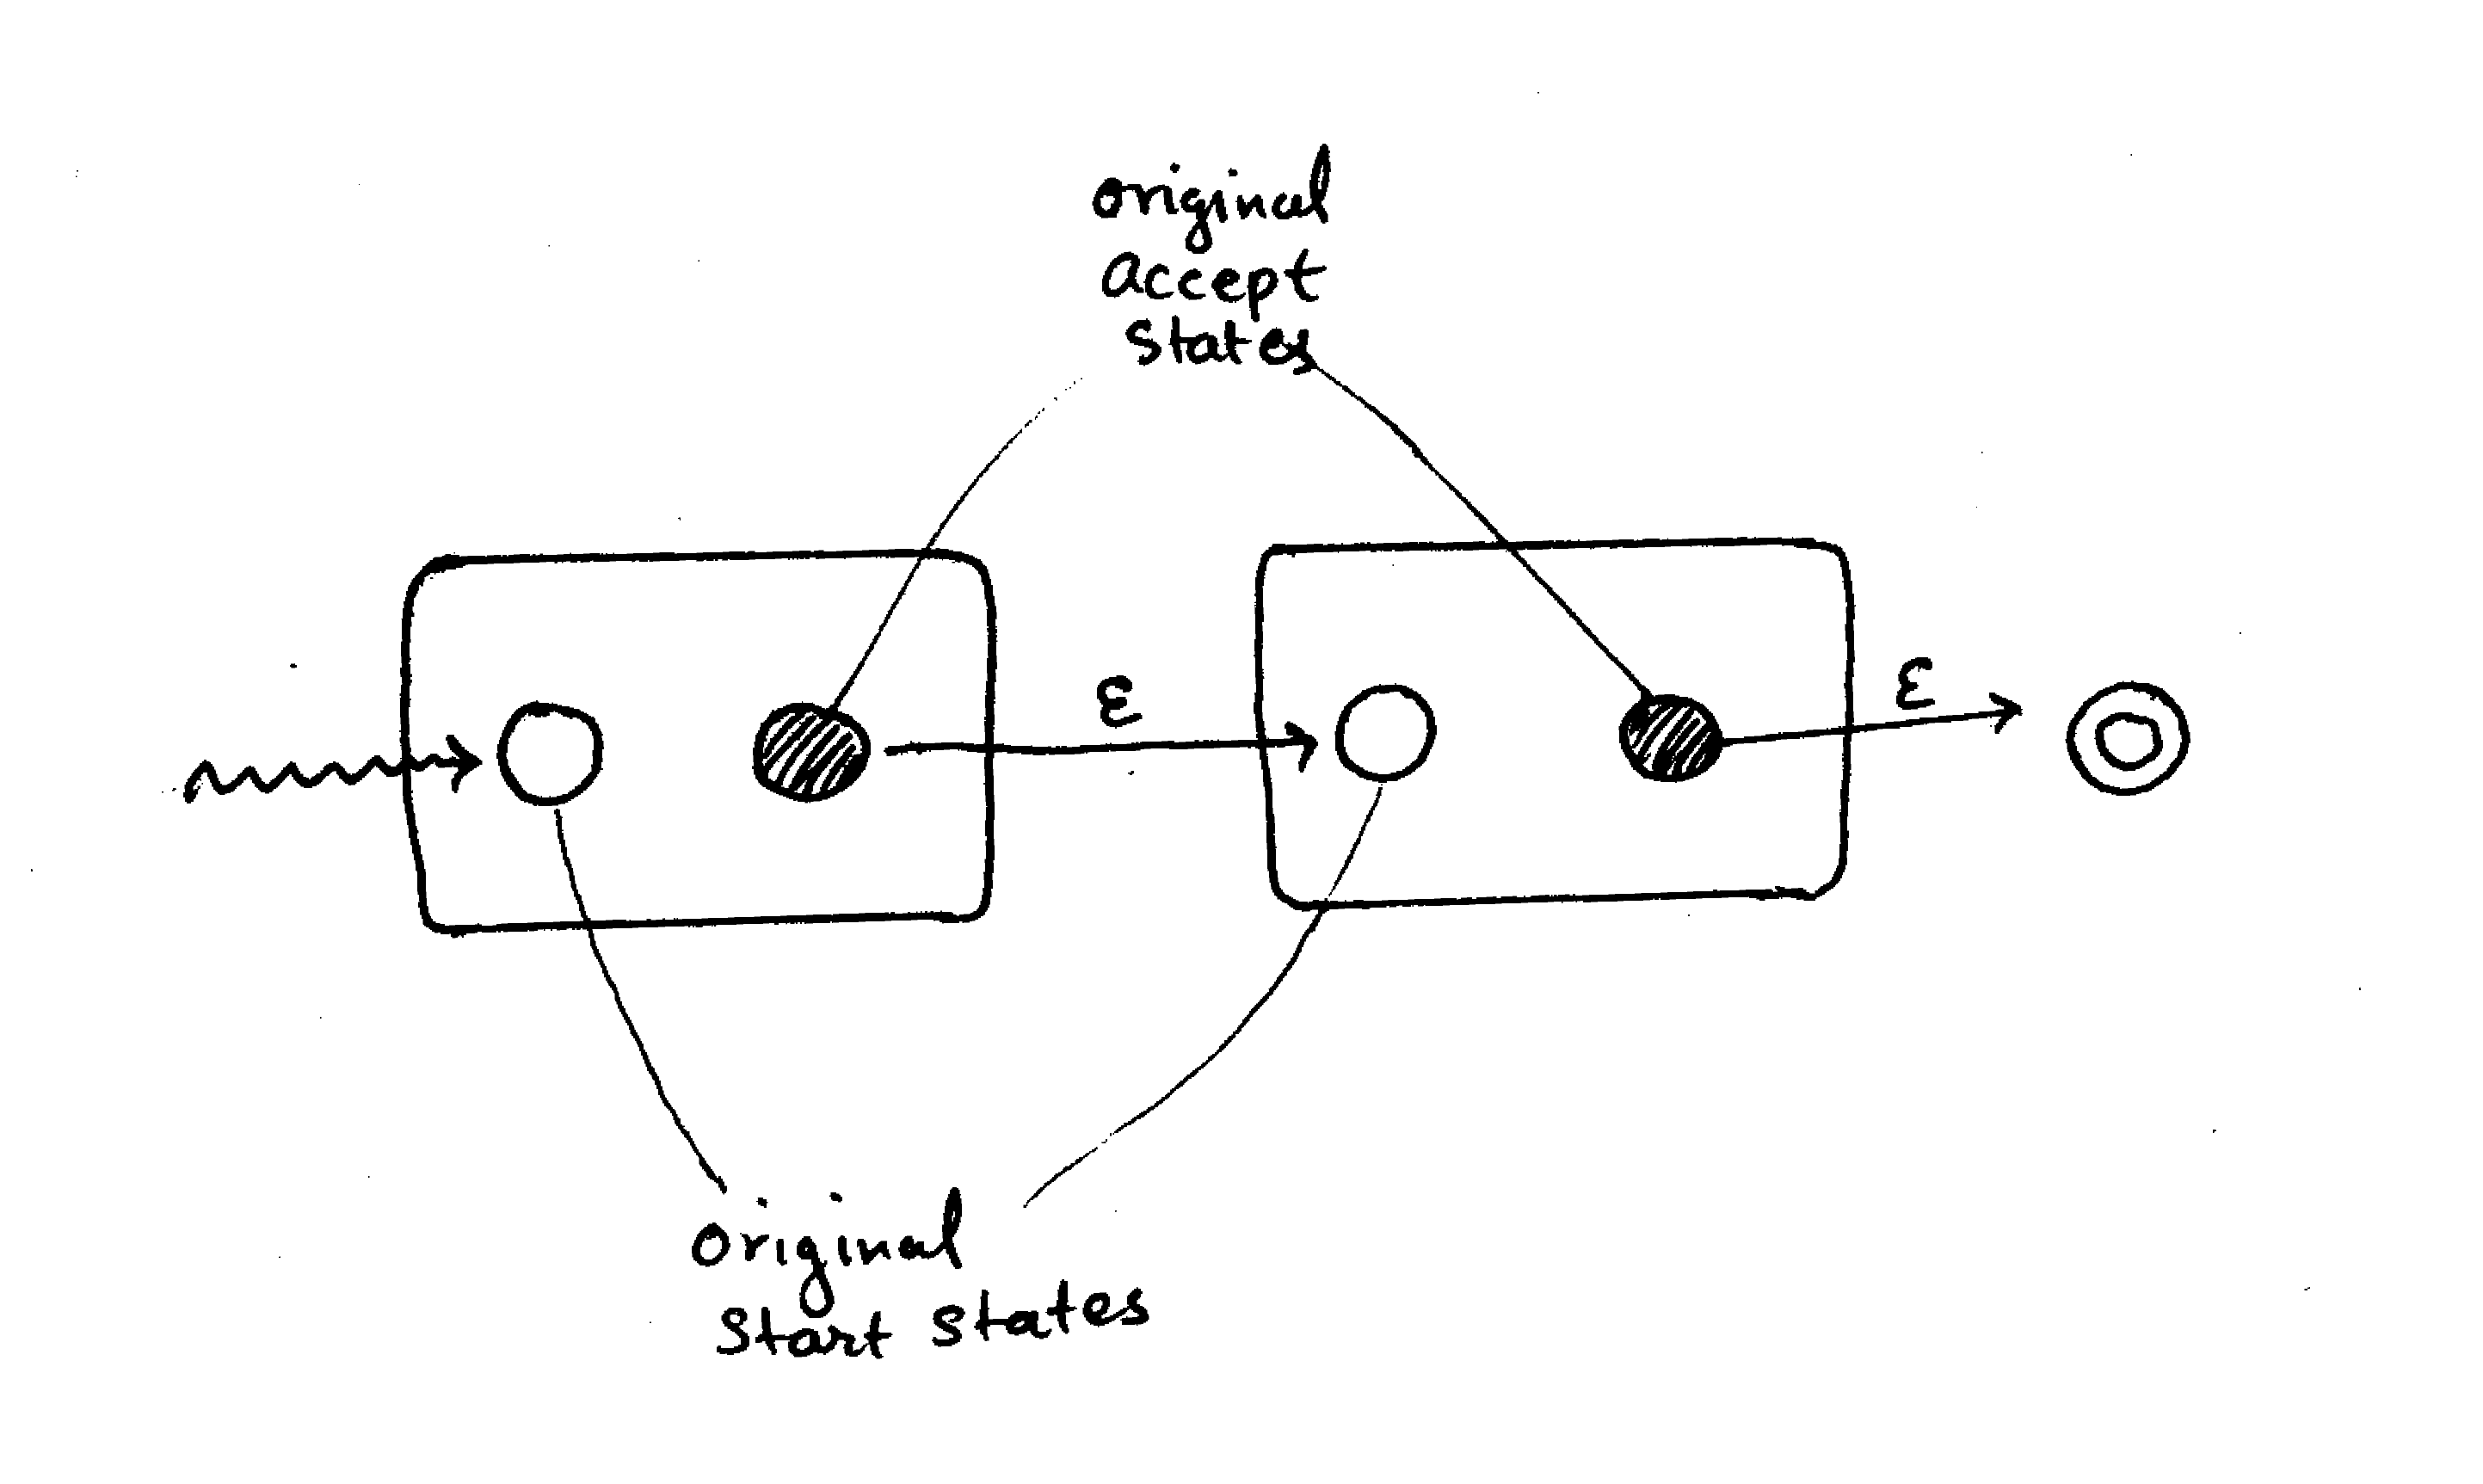
\includegraphics[scale=0.2]{resources/1-8.pdf}
    \end{center}

    If $r_1$ and $r_2$ are two regular expressions corresponding to
    $M_1$ and $M_2$ (structural induction hypothesis) then we may
    construct an automaton which accepts $r_1 \vee r_2$ as follows.
    Draw the two automata $M_1$ and $M_2$ side by side, create a new
    start state and accept state, and draw $\varepsilon$-arrows from
    the new start states to the old ones, and from the old accept
    states to the new ones. Tracing through the figure shows that a
    string is accepted by the new automaton if and only if it was
    accepted by $M_1$ or $M_2$; this is what it means to be in the
    union $L(r_1) \cup L(r_2) = L(r_1\vee r_2)$.

    \begin{center}
        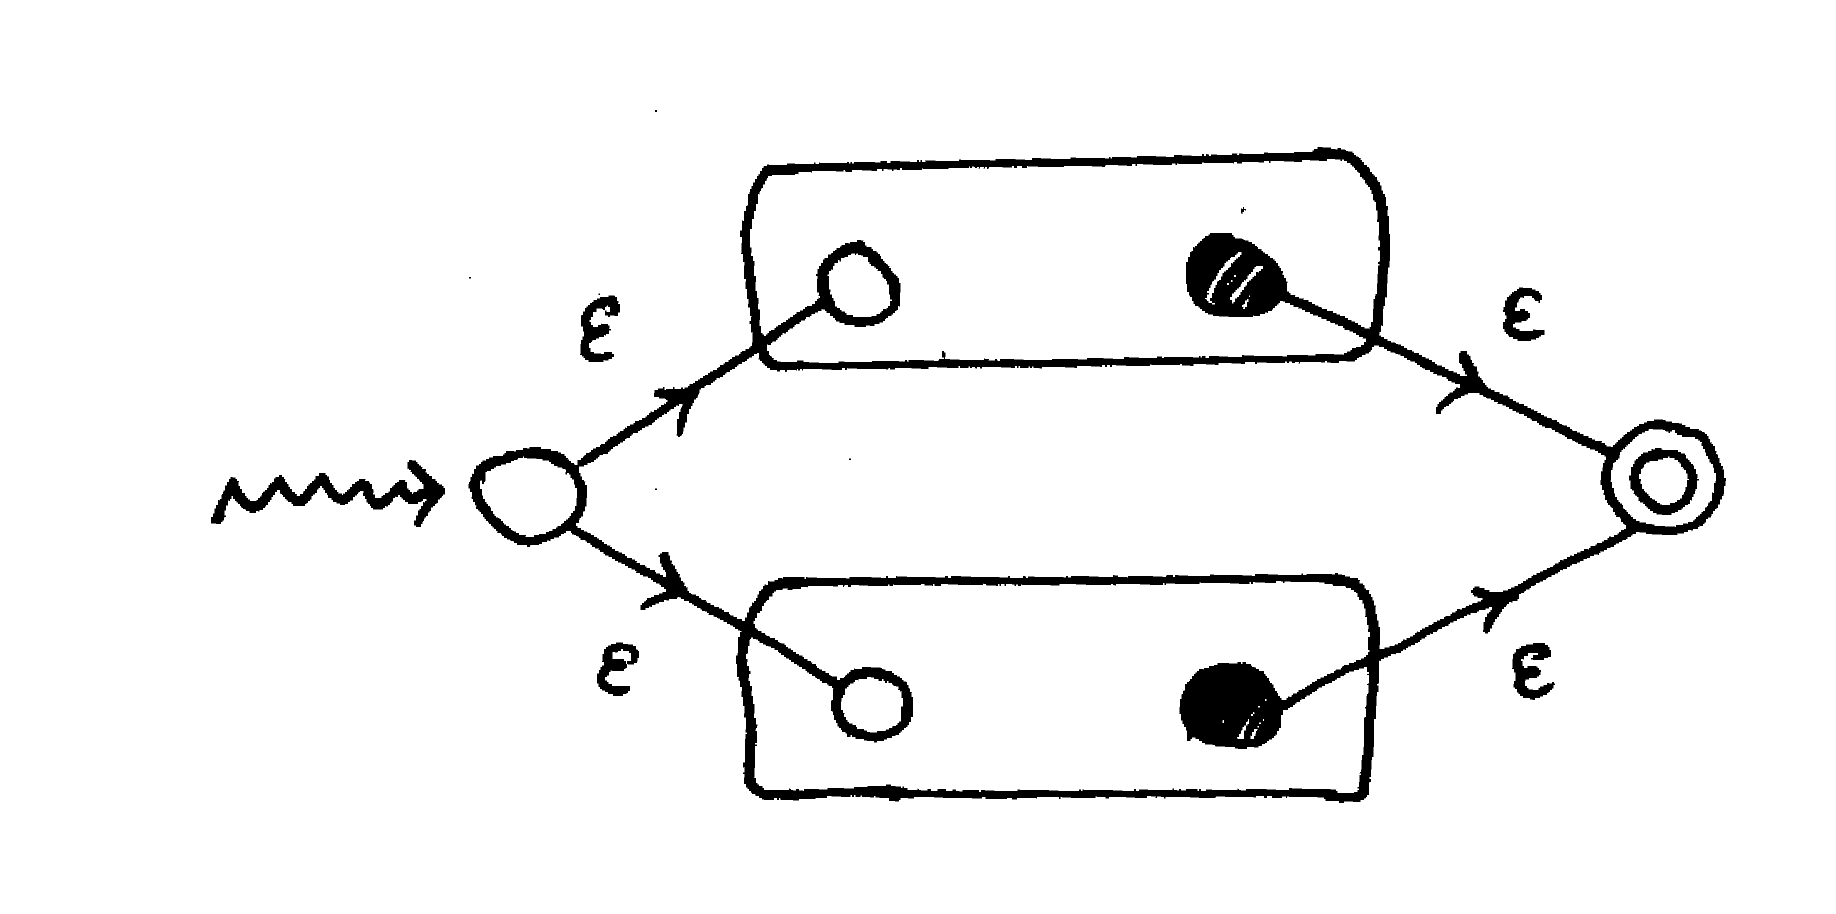
\includegraphics[scale=0.2]{resources/1-9.pdf}
    \end{center}

    This completes the proof that (d) $\Rightarrow$ (b).

    Finally, we must prove that (b) $\Rightarrow$ (a). Let $S$ be the
    state set of the given nondeterministic automaton $M$. If $X
    \subset S$, we consider the closure $\overline{X}$ of $X$ with
    respect to the $\varepsilon$-topology.  We define the required
    deterministic automaton $M'$ as follows.  The state set $S'$ is
    the set of all $\varepsilon$-closed subsets of $S$. Thus the new
    automaton has as states \emph{collections} of states from the old
    automaton. If $X$ is a state in $M'$ and $x\in A$ then we put
    \(\mu(X,x) := \) the $\varepsilon$-closure of the set of all
    targets of arrows in $M$ with source in $X$ and labelled with $x$.
    The new start state is the $\varepsilon$-closure of the original
    set of start states and the new accept states are those which
    contain an old accept state.

    To see that the new deterministic automaton $M'$ accepts the same
    language as the given nondeterministic automaton $M$, consider a
    string accepted by $M$. This string corresponds to a particular
    path $P$ in $M$. We must show that $P$ uniquely corresponds to a
    path $P'$ in $M'$. $P$ gives rise to such a $P'$ for the following
    reasons:

    (1) the ambiguity in the start state goes away by definition of
    the start state of $M',$

    (2) the transition \emph{relation} in $M$ becomes a transition
    \emph{function} in $M'$ by the definition of $\mu(X,x)$, possibly
    with $\varepsilon$-transitions, but then

    (3) the $\varepsilon$-transitions go away because $\mu$ is defined
    by means of the closure with respect to the
    $\varepsilon$-topology.

    Upon passing from $P'$ back to $P$ it is clear that $P
    \leftrightarrow P'$ is a bijection.
\end{proof}

\begin{eg} This example is taken from Sipser, page 57ff. The first
    figure is a nondeterministic automaton and the second figure is
    the corresponding deterministic automaton.

    \begin{center}
        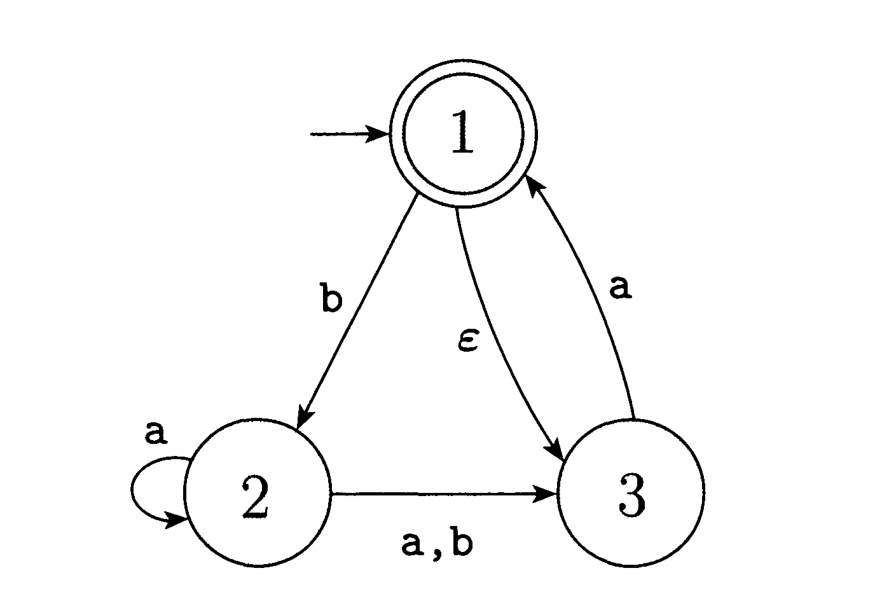
\includegraphics[scale=0.4]{resources/sipser1.pdf}
    \end{center}

    \begin{center}
        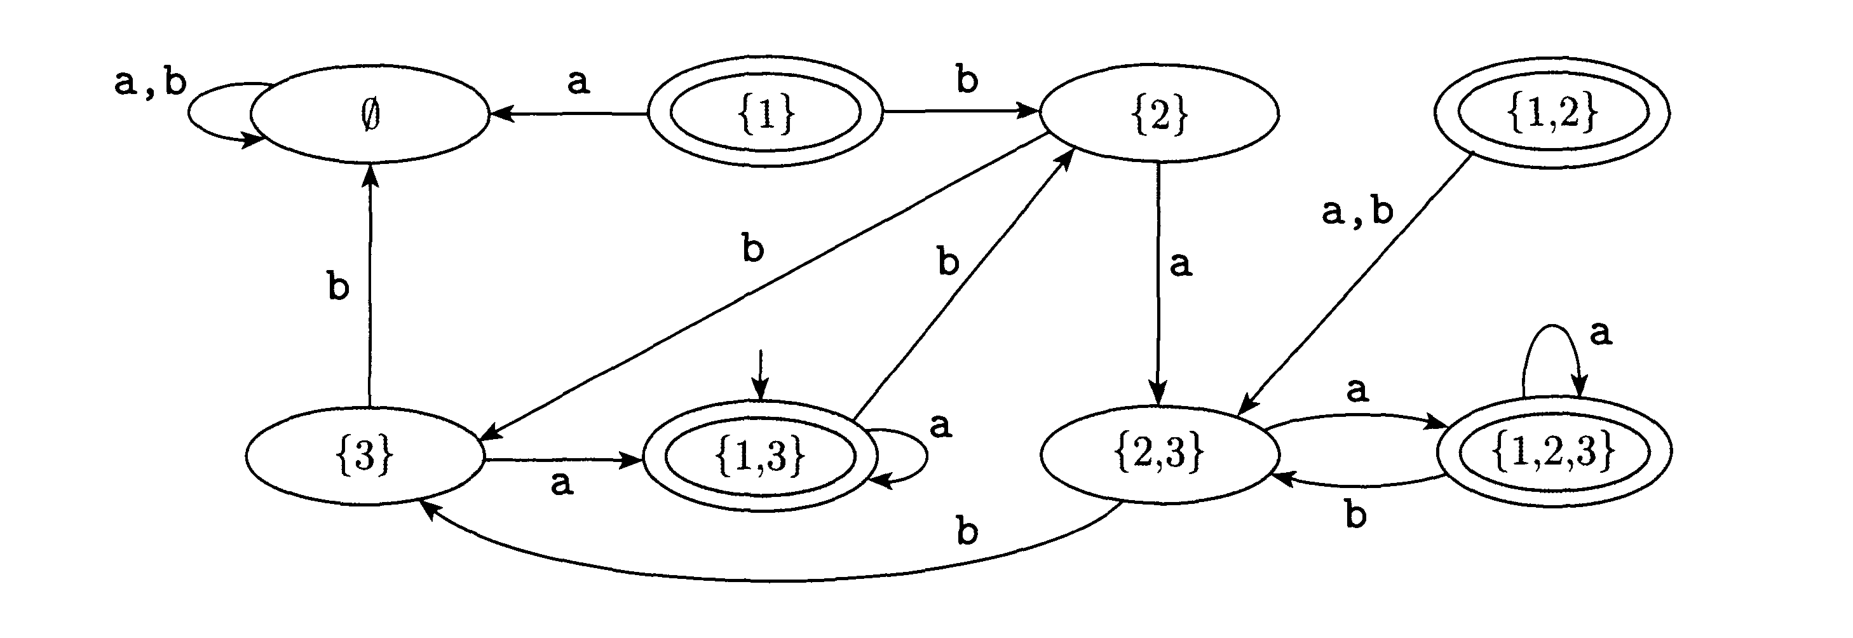
\includegraphics[scale=0.4]{resources/sipser2.pdf}
    \end{center}
\end{eg}

\begin{thm}[reversal] If $L$ is a regular language over an alphabet
    $A$ then the language consisting of the strings in $L$ written in
    the reverse order is also regular.
\end{thm}
\begin{proof} Let $M$ be a nondeterministic automaton accepting $L$
    and form the automaton $M'$ from $M$ by reversing all arrows and
    interchanging the set of start states with the set of accept
    states. We have crucially used the definition of nondeterminism;
    there must be allowed more than a single start state for this
    construction to work.
\end{proof}

\begin{thm}[Myhill-Nerode] Given a language $L$ over an alphabet $A$
    consider the following equivalence relation on $A^*$. We define $w \sim w'$
    iff \[ \forall u\in A^*:\, wu\in L \Leftrightarrow w'u \in L.\]
    Then $L$ is regular iff $A^*$ is partitioned into only finitely
    many equivalence classes under this relation.
\end{thm}
\begin{proof} First suppose that the set of equivalence classes is
    finite. Define an deterministic automaton $M$ with state set the set of
    equivalence classes. Write $[w]$ for the equivalence class, and
    also state of $M$, corresponding to $w\in A^*$. Put $[w]x :=
    [wx].$ We define the start state to be $[\varepsilon]$ and the
    accept states are the $[\ell ]$ such that $\ell \in L$. Then $M$
    accepts $L$.

    Conversely, suppose that $L$ is regular. Then it is given by some
    deterministic automaton $M$, and we assume without loss that $M$
    has no inaccessible states. Given a state $s$, choose a string
    $w_s\in A^*$ which takes the start state to $s$, and then consider
    the equivalence class of $w_s$. This class is independent of the
    choice of $w$ by the definition of the equivalence relation, so
    that the map $s\mapsto [w_s]$ is well defined. Now, given $v\in
    A^*$, put $s := \mu(s_0,v)$. Then we have that $v\sim w_s$
    i.e.~$[v] = [w_s]$.  Thus we have produced a surjective map from
    the finite set of states to the set of equivalence classes.
\end{proof}

\begin{rem} The first part of the preceeding proof shows that for a
    given regular language $L$ there is a unique minimal deterministic
    automaton accepting it.
\end{rem}

\begin{defn} If $L$ is a language over $A$, the \emph{prefix closure}
    of $L$ is the set \[L_{\text{pre}} := \{w \in A^* : w \text{ is a
    prefix of some } \ell \in L \}.\] If $L=L_{\text{pre}}$ then we
    say that $L$ is \emph{prefix closed}. Note that since the empty
    string $\varepsilon$ is a prefix of any string, it follows that a
    prefix closed language must contain the empty string.
\end{defn}

\begin{thm}[prefixes] Let $L$ be a regular language. Then the prefix
    closure of $L$ and the largest prefix closed sublanguage of $L$
    are both regular languages.
\end{thm}
\begin{proof} Let $M$ be a deterministic automaton accepting $L$. As
    usual, we assume that $M$ is normalized. Now construct $M'$ by
    turning every non-failure state of $M$ into an accept state. Then
    $M'$ accepts precisely the prefix closure of $L$.

    Next, construct $M''$ from $M$ by removing all non-accept states
    and all arrows either into or out of such a non-accept state. (In
    case the start state was not an accept state, then $M''$ has no
    start state; but in this case, the nullstring is not in $L$ so
    that $L$ has no prefix closed subsets.) Then $M''$ accepts the
    largest prefix closed sublanguage of $L$.
\end{proof}

\begin{defns} Let $A$ and $B$ be alphabets and let $f: A\rightarrow B$
    be a map. Then there exists a unique extension of $f$ to a monoid
    homomorphism $f^*: A^*\rightarrow B^*$. (We will discuss this in
    much greater detail in the sequel.) Given a language $L_A$
    over $A$, the \emph{image} of $L_A$ under $f$ is defined to be
    $f^*(L_A)$. If $L_B$ is a language over $B$ then the \emph{inverse
    image} or \emph{preimage} of $L_B$ is defined to be
    $(f^*)^{-1}(L_B)$.

    Now suppose that $f$ is a map from $A$ to the set of regular
    expressions over $B$. In this case, $f$ is called a
    \emph{substitution.} To define the image of $L_A$ under $f$ we
    proceed as follows. Extend $f$ to a monoid homomorphism from $A^*$
    to the set of regular languages over $B$ and put \[f(L_A) :=
    \bigcup_{u\in L_A} f(u).\]
\end{defns}

\begin{lem} Let $L_A$ be a regular language over $A$ and $L_B$ a
    regular language over $B$. Given $f : A \rightarrow B$ or $f:
    A\rightarrow B^*$ we have that \(f(L_A)\) resp.~\(f^{-1}(L_B)\) are
    regular languages over $B$ resp.~$A$. Given a substitution $f$,
    the image $f(L_B)$ is a regular language over $B$.
\end{lem}
\begin{proof} Let $M_A$ be a deterministic automaton accepting $L_A$.
    Replace each arrow in $M_A$ with an arrow labelled by $f(a)$. This
    gives a new automaton over $B$ which accepts $f(L_A)$; note well
    that this new automaton is generalized.  But that is sufficient to
    prove regularity of the image.

    Let $M_B$ be a deterministic automaton over $B$ accepting $L_B$.
    Define a deterministic automaton over $A$ with the same states as
    $M_B$. Given a state $s$ and $a\in A$, put $sa := sf(a)$. This new
    automaton accepts $f^{-1}(L_B)$.
\end{proof}

\begin{thm}[pumping lemma] Let $L$ be a regular language. Then there
    is a number $n>0$ such that any $x\in L$ of length $ \ge n$ is of the
    form $x=uvw$ with $|v|>0$ and $uv^iw\in L$ for all $i\ge 0$.
\end{thm}
\begin{proof}
    Let $n$ be the number of states in a deterministic automaton
    accepting $L$. If an accepted string $x$ has length $\ge n$ then
    it must visit some state twice (pigeonhole principle) and
    therefore is has a substring $v$ whose corresponding path of
    arrows forms a loop. Traversing this loop $i$ times gives the
    result.
\end{proof}

\begin{ap}[Regular Expressions in Practice]
    Go to \url{http://regexpal.com/} and click the checkbox which says
    \verb|^$ match at line breaks|. Copy any paste any text (for
    instance something from Wikipedia or some news website) into that
    site\footnote{You don't have to go to any website to try out
    regular expressions: the Unix command line tools \texttt{grep} or
    \texttt{ack} can be used to search text matching a given regular
    expression.}. For example, I have input the following words from
    my \texttt{/usr/share/dict/words} to that site

\begin{verbatim}
        craniums
        crank
        crank's
        crankcase
        crankcase's
        crankcases
        cranked
        cranker
        crankest
        crankier
        crankiest
        crankiness
        crankiness's
        cranking
        cranks
        crankshaft
        crankshaft's
        crankshafts
        cranky
        crannied
        crannies
        cranny
\end{verbatim}

Next, I have tried out the searches

\begin{verbatim}
        c.*n
        co
        ank
        c.*iu
        c..nn
        ^c
        n$
        n*
        .
        ..
        ....
\end{verbatim}

In the practice of computer programming the notion of regular
expression has a somewhat distinct, but closely related, meaning to
the one we have defined in these notes. In computer programming, a
regular expression is a pattern made from letters, numbers, and the
special characters
\begin{center}
\verb|^  $  .  * ( )|
\end{center}

This is a substantial simplification of the actual notion of regular
expression, but it conveys the idea. The meanings of the special
symbols are as follows. Any string of letters and numbers is a regular
expression. Let x stand for a regular expression. Then
\verb|^|\texttt{x} accepts those strings which start with a string
matching \texttt{x}.  \texttt{x\$} accepts those strings ending in
\texttt{x}. Let \texttt{y} be another regular expression. Then
\texttt{x.y} accepts all those strings with prefix matching
\texttt{x}, followed by any single character, and with suffix matching
\texttt{y}. The expression \verb|.| alone matches any single
character. \verb|x*| matches any number of repetitions of strings
matching \texttt{x}. Parentheses denote grouping as in an algebraic
expression.

Now, given a regular expression in the sense of Definition
\ref{regexdef}, we see how to construct a regular expression in the
computer programming sense. To construct a pattern which searches for
those strings in $L(r \vee s)$ we simply input as a search pattern
\texttt{rs}. For $L(r^*)$ we search for \verb|r*|.

Thus we see that a regular expression in the sense of computer
programming searches for those substrings of a given piece of text
which are in the language accepted by a regular expression in the
sense of Definition \ref{regexdef}.
\end{ap}

